\documentclass[11pt]{extarticle}
\usepackage{manualdoprofessor}
\usepackage{fichatecnica}
\usepackage{lipsum,media9}
\usepackage[justification=raggedright]{caption}
\usepackage[one]{bncc}
\usepackage[araucaria]{../edlab}
\usepackage{marginnote}
\usepackage{pdfpages}
%\usepackage[printwatermark]{xwatermark}
%\newwatermark[pagex=2]{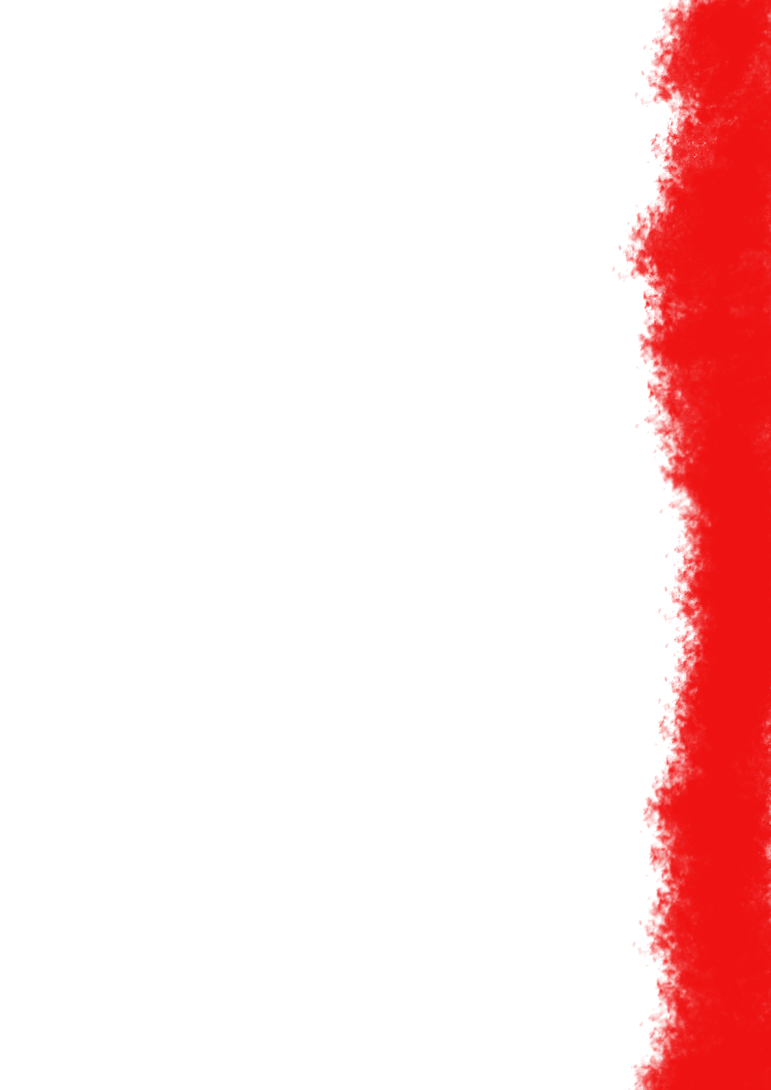
\includegraphics[scale=3.3]{watermarks/test-a.png}}	% página específica
%\newwatermark[oddpages]{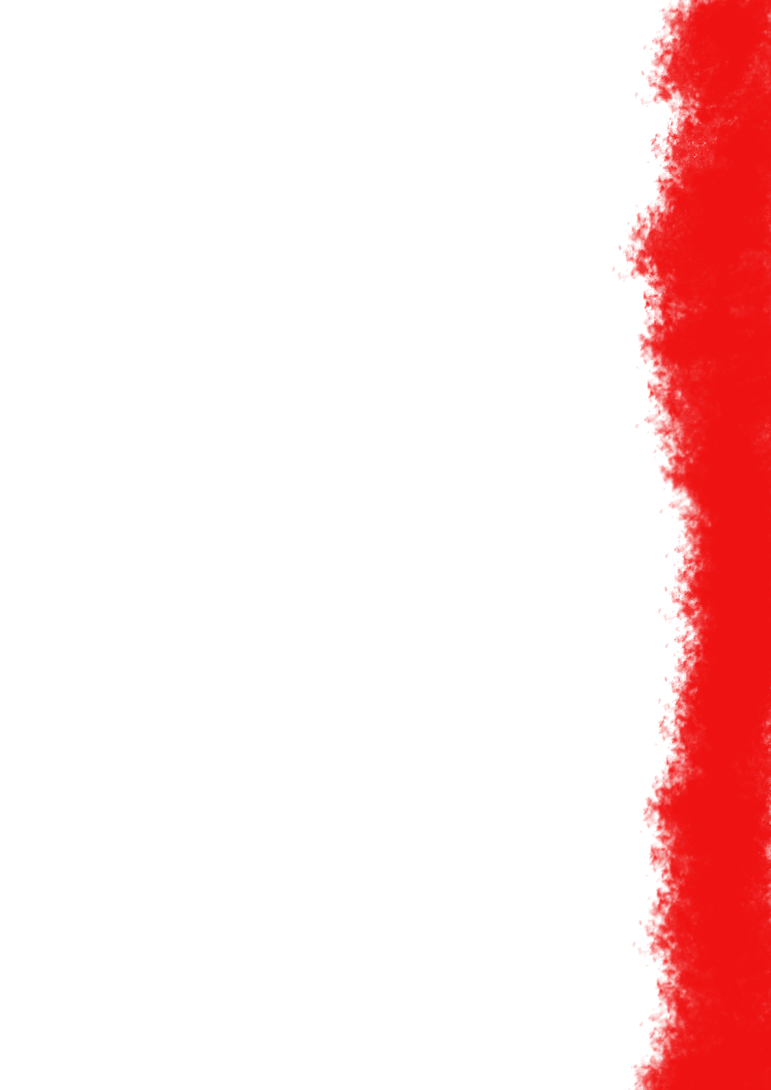
\includegraphics{watermarks/test-a.png}}			% páginas ímpars
%\newwatermark[evenpages]{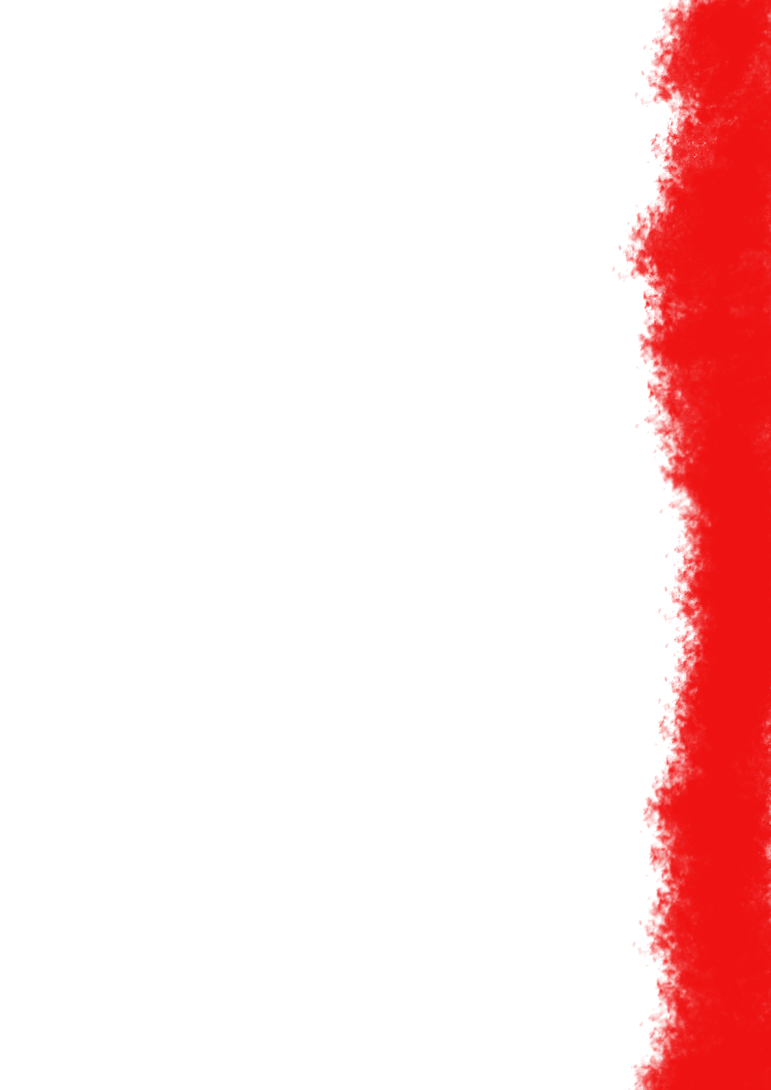
\includegraphics{watermarks/test-a.png}}			% págimas pares
%\newwatermark[allpages]{\includegraphics[scale=1]{watermarks/001.png}}

%\pagecolor{cyan!0!magenta!10!yellow!28!black!28!}

\newcommand{\AutorLivro}{Flávia Savary}
\newcommand{\TituloLivro}{Caminhando, eu vou!}
\newcommand{\Genero}{Conto; crônica; novela}
%\newcommand{\imagemCapa}{./pdf/capa.jpg}
\newcommand{\issnppub}{978-65-99441-24-0}
\newcommand{\issnepub}{978-65-99441-27-1}
% \newcommand{\fichacatalografica}{PNLD0001-00.png}
\newcommand{\colaborador}{Renier Silva}

\begin{document}

\title{\TituloLivro}
\author{\AutorLivro}
\def\authornotes{\colaborador}

\date{}
\maketitle

%\begin{abstract}\addcontentsline{toc}{section}{Carta ao professor}
%\pagebreak

\tableofcontents


\begin{abstract}

Esperamos, com este material, auxiliar os professores no trabalho com os alunos 
do Ensino Fundamental \textsc{i} em sala de aula. \textit{Caminhando, eu vou!} foi publicado
pela primeira vez em 2007 e traz a história de um retirante e seu cachorro, Severino e Eusébio que,
no meio da caatinga, veem a paisagem mudar repentinamente e se transformar num deserto.
Encontram um extenso grupo de pessoas lideradas por um homem, Moisés, que também fogem de uma situação 
ruim em busca de algo melhor. Trata-se de uma aproximação entre os retirantes nordestinos
e a passagem bíblica da fuga do povo hebreu para Canaã. 

Flávia Savary, a autora, é conhecida por seu trabalho com a literatura para
os mais diversos públicos. Ela consegue tratar de temas sérios como as migrações
de uma forma acessível, por exemplo, para os alunos do Ensino Fundamental \textsc{i},
ao se valer de recursos narrativos que flertam com o universo fantástico. 

Esperamos, professor ou professora, que este material sirva como um guia 
para seu trabalho em sala de aula. Já contamos, no entanto, com as as adaptações,
que surgirão organicamente na recepção de nossa proposta por vocês, que possuem 
trajetórias e escolhas didáticas específicas, bem como no contato com os 
alunos, que tanto têm a oferecer para o enriquecimento da experiência didática.

Boa aula!

\end{abstract}

\section{Sobre o livro}

%550 caracteres
\paragraph{O livro} 

\textit{Caminhando, eu vou!} é uma narrativa curta que conta a história de duas personagens, Severino e Eusébio,
seu cachorro companheiro, que caminham no meio da caatinga em direção ao litoral em busca de uma vida melhor, 
longe da seca. Constituem, assim, o retrato do retirante nordestino. 
No meio do caminho, encontram aquilo que parece ser uma miragem: um extenso grupo de pessoas também em marcha,
mas guiadas por um líder, Moisés. Trata-se dos hebreus, em fuga do Egito, onde eram escravizados
pelo Faraó. O sertanejo e seu cão acompanham de perto e participam do episódio miraculoso, narrado na Bíblia,
da abertura dos mares, que garante a salvação aos que escapavam e a derrota aos que os perseguiam. 

Antônio Conselheiro e Moisés, caatinga do Nordeste e deserto do Egito, 
Faraó e senhor de engenho. Unidos pelo contexto de fuga em direção a uma vida melhor, mais próspera e com mais liberdade,
as histórias do retirante nordestino e a dos hebreus em fuga do Egito se encontram nessa pequena narrativa que
conjuga um assunto tão caro à história da humanidade e cada vez mais à ordem do dia:
o direito de ir e vir, de imigrar e recomeçar a própria história e a de um grupo. 


\section{Sobre o autor}

\paragraph{Flávia Savary}

%inserir foto do autor à margem 

Flávia Savary é escritora, ilustradora e dramaturga, nascida no Rio de Janeiro em setembro de 1956. 
Formada em Letras pela Universidade Federal do Rio de Janeiro, trabalha com literatura desde 1979.
Como ilustradora e artista plástica, participou de várias exposições nacionais e internacionais.
Ganhou cerca de 80 prêmios literários, no Brasil e no exterior. Tem poemas, peças teatrais, crônicas e narrativas de ficção 
(para público infantil, juvenil e adulto) publicados em mais de quarenta antologias.
Dentre seus trabalhos, podemos listar: \textit{A roupa nova do arco-da-velha}, \textit{O herói}, \textit{Lendas da Amazônia... e é assim até hoje}, \textit{Laura levou o vento}, \textit{O mundo muda se a gente ajuda}, \textit{A rosa que gira a roda},
\textit{Vinte cantos de sereia}.


\section{Sobre o gênero}

%55 caracteres
\paragraph{O gênero} O gênero deste livro é \textit{conto; crônica; novela}. 

%596 caracteres

\paragraph{Descrição} O que define um gênero narrativo é o fato de, não importa
qual seja sua forma, eles \textit{contarem uma história}.
As especificidades do \textit{como} esta história será contada é que
qualificaram os tipos de gênero narrativo, que podem ser: conto, crônica, novela,
epopeia, romance ou fábula. 

Toda narrativa possui, necessariamente, um narrador, uma personagem, um enredo,
um tempo e um espaço. O narrador, ou narradora, pode ser onisciente, literalmente
\textit{que tudo sabe}, observador ou personagem --- categorias que não são excludentes.
O discurso elaborado por este narrador ou narradora pode ser direto, indireto ou indireto livre 
--- ou seja, ele ou ela pode aparecer mais diretamente ou mais indiretamente; no último caso,
sua voz se mistura à das personagens da história.

O narrador \textbf{não é necessariamente} a voz do autor. É errada a afirmação
de que o autor fala através do narrador de uma história. É bastante comum,
há algum tempo na história literária, sobretudo desde os pré-modernistas, que 
o narrador represente justamente o contrário do que pensa o autor. Neste caso, 
utilizam-se elementos como a \textbf{ironia} para sugerir que o autor \textit{não é confiável}.

Já as personagens variam quanto a sua \textbf{profundidade}. Há personagens planas, ou
personagens-tipo, e personagens redondas, ou complexas. Personagens planas
são facilmente repetíveis pois se amparam em lugares-comuns da cultura, como
o vilão, o herói, a vítima, o palhaço, tudo isso com marcações de gênero e espécie ---
o herói tradicionalmente é um homem, a vítima, uma mulher, e o vilão, uma figura que 
se afasta da humanidade por alguma razão, às vezes sobrenatural. 
Personagens redondos, por outro lado, estão mais próximos das \textit{pessoas reais}.
Uma personagem complexa pode ser, em um dado momento da narrativa, vilã, e em 
outro, heroína. É importante notar como as visões de mundo, um traço cultural e 
portanto relativo, influenciam na caracterização das personagens, planas 
ou redondas, de uma história.

O tempo de uma narrativa pode ser cronológico ou psicológico.
No tempo cronológico, o enredo segue a ordem ``normal'' dos acontecimentos,
aquela marcada pelo relógio e pelo calendário. Os acontecimentos vêm um após o 
outro, e se delimita muito bem \textit{passado}, \textit{presente} e \textit{futuro}.
Já no tempo psicológico, segue-se uma ordem \textit{subjetiva} dos acontecimentos, 
e portanto, \textit{não linear}, já que a influência emocional e psíquica 
da subjetividade afeta a racionalidade do tempo cronológico. 

O espaço, por fim, é o lugar onde se passa a narrativa. Dependendo do caso, 
ele pode funcionar mais como um pano de fundo, sem muita interferência
no enredo, ou mais ativamente, aproximando-se das características das personagens
e influenciando no desenrolar da trama. 

O último aspecto de um gênero narrativo que podemos abordar é sua 
\textit{extensão}. Dentre os elementos que distinguem um subgênero 
de outro, é fundamental o tamanho da história: uma crônica e um conto são \textit{necessariamente}
curtos, ao passo que uma epopeia e um romance são longos. Uma novela
está no ponto intermediário entre um romance e um conto.
Ainda poderíamos falar dos registros de cada subgênero: 
a epopeia é originalmente um subgênero \textit{oral}, versificado, e metrificado,
já o romance é tradicionalmente \textit{escrito} em prosa. 
Desde meados do século \textsc{xviii}, no entanto, o estabelecimento
dos gêneros e subgêneros narrativos torna-se cada vez menos rígido,
com as características cada vez mais fluidas e intercomunicativas.

Como o presente livro contém uma narrativa \textit{curta},
finalizamos com as palavras de Luiza Vilma Pires a respeito do
subgênero:

\begin{quote}
sob o nome de narrativa curta, estão situadas obras que apresentam uma trama 
um pouco mais complexa, que ocorre em diversos espaços e em uma temporalidade 
que pode ser de vários dias, semanas ou meses. Entretanto a função das ilustrações 
continua as mesmas, são complementares à história e contribuem para sua compreensão. 
Os temas relacionam-se a vivência infantis (brincadeiras, passeios, pequenas aventuras), 
a aspectos ligados à interioridade das personagens (busca de identidade, insegurança, 
medos) ou a relações interpessoais (desentendimentos familiares, entre amigos, solidariedade).\footnote{“Narrativas infantis”, de Luiza Vilma Pires Vale. In \textsc{saraiva}, J. A. (Org.) \textit{Literatura e alfabetização: do plano do choro ao plano da ação}. Porto Alegre: Artmed, 2001.} 
\end{quote} 

\section{Atividades}

\subsection{Pré-leitura}

\BNCC{EF35LP10}
\BNCC{EF35LP11}
\BNCC{EF03HI08}
\BNCC{EF03GE11}
\BNCC{EF03HI07}
\BNCC{EF03HI11}

\paragraph{Atividade 1}

\paragraph{Tema} Imigração e busca por uma vida melhor.

\paragraph{Conteúdo} Compreensão do fenômeno social e cultural da imigração ao redor
do mundo.

\paragraph{Justificativa} O livro que o professor ou a professora tem em mãos trata de um assunto caro a muitas pessoas no mundo inteiro: o deslocamento espacial em busca de uma vida melhor. Desde a época do povo hebreu que fugiu do Egito para
ir atrás de sua Terra Prometida, ou dos Tupi e Guarani, na busca da Terra Sem Mal, passando pelos retirantes 
nordestinos na fuga da seca e da tirania dos coronéis, até hoje, com os imigrantes em situação de refúgio por 
conta de questões políticas e econômicas. O desejo por um lugar com mais qualidade de vida, fartura e prosperidade 
para si e para os seus faz parte da condição humana. Como este é o assunto principal do livro que será trabalhado em sala, é importante que seja feita
uma introdução neste primeiro momento. 


\paragraph{Metodologia} Comece a aula perguntando aos alunos:

\begin{itemize}
\item Onde eles nasceram?
\item Onde seus pais nasceram?
\item Onde seus avós nasceram?
\item Onde seus bisavós nasceram? 
\end{itemize}

É provável que as duas últimas perguntas encontrem dificuldades para serem respondidas
devido à maior distância em relação às crianças. 
Neste ponto, você, professor ou professora, pode contar a história de sua família,
respondendo às mesmas questões. 
Como o Brasil é um país de povos em movimento, é muito comum que os pais e avós venham de regiões diferentes
do mesmo país, ou mesmo de outros. Relate os motivos que influenciaram suas decisões de partir:
busca de emprego, perseguição política, motivos pessoais etc.


\paragraph{Atividade 1.2} 

Depois que você tiver compartilhado a história de sua família ou alguma outra próxima a você com os alunos,
e eles tiverem feito o mesmo, introduza o tema das duas migrações que estruturam a narrativa que será lida:
os retirantes nordestinos na fuga da seca, rumo às capitais no litoral ou ao Sudeste, e o povo hebreu
em busca da Terra Prometida no Egito.
Você pode começar, com o auxílio do professor ou professora de História, com uma contextualização 
histórica do Egito Antigo. 

A chegada dos hebreus ao Egito teria coincidido com o período em que a região 
estava sob domínio dos hicsos, um povo de origem semita, como os hebreus. Isso possibilitou que os hebreus 
se estabelecessem no território egípcio sem problemas, chegando até a ocupar posições de proeminência na 
administração do Egito. Após a expulsão dos hicsos, os hebreus teriam sido punidos pela colaboração com os 
invasores. Os hebreus, escravizados pelos egípcios, conseguiram sua libertação por meio de Moisés, em 
aproximadamente 1300 a.C.

Pergunte aos alunos se eles já haviam ouvido falar nesta história. É possível que alguns deles, 
por conta de uma formação religiosa, a conheçam em partes. Incentive-os a compartilhar
apontamentos, mas esteja sempre atento ou atenta a mediações quando julgar necessário.

Já os retirantes provêm de classes sociais menos favorecidas e procediam principalmente do interior do 
Nordeste, região do polígono das secas dominada pelos coronéis, que expulsavam os habitantes locais de suas antigas
propriedades e propunham uma forma de trabalho equivalente à servidão. 

Por fim, apresente aos alunos a obra ``Os retirantes'' do artista visual brasileiro Cândido Portinari,
que representa uma família de retirantes. Pergunte quais são os principais elementos que eles encontram
na imagem. Ressalte a falta de expressões faciais, sinais físicos de desnutrição, ossos de animais mortos
no chão, terra seca, aves carniceiras no céu etc.

\Image{Quadro ``Os retirantes'' de Cândido Portinari. (Acervo do \textsc{masp}.)}{PNLD2023-026-01.jpg}


\paragraph{Atividade 1.3}

No último momento da pré-leitura, indique outras obras que tratem do mesmo tema. 
\textit{O quinze}, de Rachel de Queiroz, \textit{Morte e vida severina}, de João Cabral de Melo Neto, 
e \textit{Vidas secas}, de Graciliano Ramos, são todos textos literários que abordam 
a jornada da busca dos retirantes por uma vida melhor. Todas essas obras foram adapatadas para o formato de quadrinhos, mais adequado para a faixa etária de seus estudantes. \textit{Vidas secas} ganhou uma adaptação ao cinema 
de Nelson Pereira dos Santos, em 1963. Caso julgue aproveitável, o professor ou a professora
pode exibir \href{https://www.youtube.com/watch?v=m5fsDcFOdwQ&t=9s}{trechos da obra}.

\paragraph{Tempo estimado} Quatro aulas de 50 minutos. 

\subsection{Leitura}

\BNCC{EF03HI01}
\BNCC{EF35LP03}
\BNCC{EF35LP05}
\BNCC{EF35LP06}
\BNCC{EF35LP19}

\paragraph{Atividade 1}

\paragraph{Tema} Verossimilhança e estrutura narrativa.

\paragraph{Conteúdo} Discussão a respeito dos conceitos de verossimilhança 
e temporalidade na estrutura da narrativa.

\paragraph{Justificativa} A verossimilhança é o que garante aparência de 
verdade a uma narrativa. Com ela, os fatos narrados não precisam ser necessariamente
reais, mas sim apresentar estrutura coerente. Há fatos reais que são inverossímeis,
e fatos narrados que são verossímeis. A compreensão deste conceito é essencial para
o estudo de literatura e formação crítica dos estudantes.


\paragraph{Metodologia} Em voz alta, leia junto à turma. Faça pequenas pausas para discussão 
acerca da \textbf{estrutura} do texto. Quanto aos personagens, pergunte:

\begin{itemize}
\item Quem são as personagens do começo da história? 
\end{itemize}

Ainda que se trate, no livro, de situações \textbf{verossímeis}, a fuga de povos 
em busca de uma vida melhor, com mais prosperidade e liberdade, há elementos 
que flertam com o \textbf{mágico} e o \textbf{fantástico} na narrativa. Logo no início, quando 
ainda estão somente o homem, Severino, e seu cachorro, Euzébio, ao perceber a 
súbita mudança da paisagem da caatinga para a de um deserto, Severino diz: 
\textit{``Só lembro de ter cochilado um tiquinho de nada pra dar trégua aos miolos 
que se cozinhavam no calorão... E apareço num lugar nunca visto!''}. E ao final 
da aventura: \textit{``Menino, será que foi um sonho que eu tive?''}.

Pergunte aos alunos:

\begin{itemize}
	\item O que parecem indicar, na narrativa, essas duas observações?
\end{itemize}

Ao fim da discussão, explique à turma que a verossimilhança garante 
a um enredo uma \textbf{aparência de verdade} ainda que os fatos
não sejam verdadeiros na realidade. Esse recurso permite que os autores
se valham da imaginação e da fantasia para criar histórias atraentes
e convincentes. Sem ele, as histórias que não fossem imediatamente
iguais aos fatos reais seriam irrelevantes.

\paragraph{Tempo estimado} Quatro aulas de 50 minutos.


\paragraph{Atividade 2}

\paragraph{Tema} Biomas e imigrações.

\paragraph{Conteúdo} Localização e comparação entre os biomas
da caatinga e do deserto, e análise das imigrações que ocorrem em cada um. 

\paragraph{Justificativa} A proximidade narrativa entre as histórias do
retirante sertanejo da caatinga e os hebreus na fuga do Egito aparece, também,
numa análise geográfica e cartográfica de ambos os casos. 
Ainda que se distingam pelas suas especificidades, a caatinga nordestina e o deserto do Saara
possuem similaridades como a secura e a inospitalidade, que os caracterizam
como lugares de transição.

\paragraph{Metodologia} 
Aproveitando o ensejo da aproximação entre \textbf{caatinga} e \textbf{deserto}, 
com a contribuição do professor ou professora de Ciências, proponha uma pesquisa acerca dos 
dois biomas, suas similaridades e diferenças.

\Image{Deserto, bioma característico da região do Egito. (CC-BY-2.0)}{PNLD2023_026_03.jpg}
\Image{Caatinga, bioma brasileiro localizado na região Nordeste. (CC-BY-2.0)}{PNLD2023_026_02.jpg}

Peça que os alunos indiquem, no mapa, onde se situam as regiões da 
caatinga nordestina, e o deserto que Moisés e seu povo atravessaram.

Por fim, pergunte aos alunos: 

\begin{itemize}
\item O que aproxima estes dois povos tão distantes espacialmente? 
\end{itemize}


\paragraph{Tempo estimado} Duas aulas de 50 minutos.  

 
\subsection{Pós-leitura}

\BNCC{EF02ER03}

\paragraph{Tema} Escrevendo a própria história.

\paragraph{Conteúdo} Escrita de uma narrativa genealógica de cada aluno,
real ou fictícia.

\paragraph{Justificativa} A escrita de uma narrativa de si ligada à própria 
linhagem familiar ajuda o indivíduo a se situar temporalmente e espacialmente
no mundo. No caso de linhagens menos claras, com lacunas e apagamentos,
a escrita a partir de pistas, baseada na verossimilhança, já estudada,
pode inclusive ser útil para elaborar criativamente estas lacunas,
com uma reverberação positiva tanto para o aluno quanto para sua família. 
\Image{Mapa dos biomas distribuídos pelo planeta. Atenção às regiões do Egito e do interior do Nordeste brasileiro.
(CC-BY-2.0)}{PNLD2023-026-04.png}

\paragraph{Metodologia} 
Após a leitura, é hora de escrever a própria história.
Retomando a conversa inicial da atividade de pré-leitura
acerca das origens familiares, os alunos devem escrever, 
individualmente, estas histórias. Para isso, eles podem
seguir o gênero narrativo, como lhes foi apresentado em
\textit{Caminhando, eu vou!}, mas também podem optar
por outros gêneros, como o cordel ou as histórias em 
quadrinhos, que comportam uma parte visual. 

Para levantamento de material para a escrita, eles devem
entrevistar seus familiares acerca do assunto \textbf{origens}
e \textbf{migrações}. De onde vêm seus pais, seus avós, seus 
antepassados, de uma forma geral? 

Quando os textos forem finalizados, os alunos podem disponibilizá-los 
num blog da turma para o acesso do restante da comunidade escolar 
e familiar. Antes disso, é importante que haja uma partilha em sala de aula.
Possivelmente, haverá histórias parecidas e mesmo origens comuns.
Deste modo, os alunos estarão trabalhando competências que dizem
respeito a noções como sociabilidade, diversidade e família na 
constituição do ``eu'' e do ``outro''.


\paragraph{Tempo estimado} Quatro aulas de 50 minutos.


\section{Sugestões de referências complementares}

\subsection{Músicas} 

\begin{itemize}
	\item \href{https://www.youtube.com/watch?v=zsFSHg2hxbc}{``Asa branca''}, baião composto por Luiz Gonzaga e Humberto Teixeira, retrata 
a situação dramática vivida pelos habitantes do sertão em épocas de seca. 

	\item Álbum musical \href{https://www.youtube.com/watch?v=wS6jzcZcc6U}{\textit{Nordeste: Cordel, Repente, Canção}}. 

\end{itemize}

\subsection{Filmes}

\begin{itemize}

	\item \textit{Vidas secas}, de 1963, de Nelson Pereira dos Santos. Adaptação para o cinema do romance homônimo
de Graciliano Ramos. Uma família de retirantes nordestinos ruma em direção à capital em busca de uma vida
melhor, longe da seca e dos abusos dos patrões. 

	\item \href{https://www.youtube.com/watch?v=xFOZxwBcUmo}{\textit{Nordeste: Cordel, Repente, Canção.}}.

\end{itemize}
\subsection{Livros}

\begin{itemize}
	\item \textit{A chegada de Lampião no inferno}, de José Pacheco da Rocha. 

O cordel continua a história de Lampião após a sua morte, narrada em \textit{Lampião... Era o cavalo do tempo atrás da besta da vida}, quando ele teria descido ao Inferno e fora recebido com assombro pelo próprio Diabo. 

	\item \textit{O Quinze}, de 1930, de Rachel de Queiroz. O romance retrata a histórica seca de 1915, vivida
pela própria autora, em sua infância. A grande seca de 1915 assolou o sertão da região Nordeste do Brasil
e provocou a mudança repentina da população das classes mais baixas para regiões mais prósperas economicamente.
Como é visto na narrativa, essa busca costumava acabar em desgraça: mortes por fome e desnutrição no meio do caminho.
\end{itemize}

\begin{itemize}
\item \textsc{sardelich}, Maria Emilia. \href{https://www.scielo.br/pdf/cp/v36n128/v36n128a09}{Leitura de Imagens, Cultura Visual e Prática Educativa}. 
In: Cadernos de Pesquisa. V.36, n.128, p.451-472, mai/ago.2006. 

Artigo acadêmico que discorre sobre a importância de trabalhar cultura 
visual na educação na sociedade contemporânea. 

\item {\textsc{pranke}}, Marha Elfrida. \href{http://centraldeinteligenciaacademica.blogspot.com/2016/04/organizacao-dos-espacos-da-sala-de-aula.html}{Organização dos espaços da sala de aula na Educação Infantil}. 

Artigo acadêmico que discorre sobre a importância da rotina e de criar ambientes dentro da sala de aula na Educação Infantil.  
\end{itemize}

\subsection{\textit{Sites}}

\begin{itemize}
\item Google Arts and Culture: \textit{Séries bíblica e retirantes de Cândido Portinari no Museu de Arte de São Paulo} (\textsc{masp}).

Fazem parte das séries obras como ``Os retirantes'', apresentada nas atividades de pré-leitura, onde se vê representada
uma família de retirantes em situação de miséria. Dentre as obras das séries, também está ``Criança morta'', representando uma
situação corriqueira no quotidiano miserável dos retirantes. 

\end{itemize}

\section{Bibliografia comentada}

\begin{itemize}
\item \textsc{brasil}. Ministério da Educação. Base Nacional Comum Curricular. Brasília, 2018.

Consultar a \textsc{bncc} é essencial para criar atividades para a turma. Além de especificar 
quais habilidades precisam ser desenvolvidas em cada ano, é fonte de informações sobre 
o processo de aprendizagem infantil. 

\item \textsc{brasil}. Ministério da Educação. Secretaria de Alfabetização. \href{http://alfabetizacao.mec.gov.br/images/conta-pra-mim/conta-pra-mim-literacia.pdf}{Conta pra mim: Guia de Literacia Familiar}. 
Brasília: \textsc{mec, sealf}, 2019. 

Este guia é voltado aos pais e oferece explicações em uma linguagem bastante acessível e detalhada as práticas de Literacia Familiar, 
como praticar leitura dialogada, como narrar histórias, como exercitar interação oral, formas de proporcionar contatos com a escrita à criança etc. 
 
\item \textsc{brasil}. Ministério da Educação. Secretaria de Alfabetização. PNA Política Nacional de Alfabetização/Secretaria 
de Alfabetização. Brasília: \textsc{mec, sealf}, 2019.

Um guia fundamental para trabalhar pré-alfabetização e alfabetização de estudantes, que ressalta a importância da Literacia e da Numeracia. 

\item \textsc{van der linden}, Sophie. Para ler o livro ilustrado. São Paulo: Cosac Naify, 2011.

Livro sobre as particularidades do livro ilustrado, que apresenta as diferenças entre o livro ilustrado e o livro com ilustração. 
\end{itemize}

\end{document}
